\documentclass[frenchb,10pt, a4paper]{report}
\usepackage{eso-pic}	% Nécessaire pour mettre des images en arrière plan
\usepackage{array}
\renewcommand{\labelitemi}{$\bullet$}
\renewcommand{\labelitemii}{$\bullet$}

\usepackage[utf8]{inputenc}
\usepackage[T1]{fontenc}
\usepackage{xcolor}
\newcommand\overmat[2]{%
  \makebox[0pt][l]{$\smash{\color{white}\overbrace{\phantom{%
    \begin{matrix}#2\end{matrix}}}^{\text{\color{black}#1}}}$}#2}
\newcommand\bovermat[2]{%
  \makebox[0pt][l]{$\smash{\overbrace{\phantom{%
    \begin{matrix}#2\end{matrix}}}^{\text{#1}}}$}#2}
\newcommand\partialphantom{\vphantom{\frac{\partial e_{P,M}}{\partial w_{1,1}}}}
\usepackage{lmodern}
\usepackage[
paper=a4paper, % Change to letterpaper for US letter
% inner=2.5cm, % Inner margin
% outer=3.8cm, % Outer margin
% bindingoffset=.5cm, % Binding offset
% top=2.5cm, % Top margin
% bottom=2.5cm, % Bottom margin
]{geometry}
\usepackage{babel}
\usepackage{tikz}
\usetikzlibrary{automata, positioning, arrows,shapes,decorations,calc,arrows.meta,fit}
\usetikzlibrary{decorations.pathmorphing}
\usetikzlibrary{decorations.pathreplacing}
\usetikzlibrary{decorations.shapes}
\usetikzlibrary{decorations.text}
\usetikzlibrary{decorations.markings}
\usetikzlibrary{decorations.fractals}
\usetikzlibrary{decorations.footprints}
\usepackage{minitoc}
\setcounter{secnumdepth}{3}
\setcounter{tocdepth}{1}
\setcounter{minitocdepth}{3}

% \tikzset{
%     -Latex,auto,node distance =1 cm and 1 cm,semithick,
%     state/.style ={ellipse, draw, minimum width = 0.7 cm},
%     point/.style = {circle, draw, inner sep=0.04cm,fill,node contents={}},
%     bidirected/.style={Latex-Latex,dashed},
%     el/.style = {inner sep=2pt, align=left, sloped}
% }
\usepackage{multirow}
\usepackage{appendix}
\usepackage{framed}
\usepackage{graphicx}
\usepackage{caption}
\usepackage{subcaption}
\usepackage{mathpazo}
\usepackage{amsmath}
\usepackage{booktabs}
\usepackage{hyperref}\usepackage{xcolor}
\usepackage[linesnumbered,ruled,vlined]{algorithm2e}
\newcommand\mycommfont[1]{\footnotesize\ttfamily\textcolor{blue}{#1}}
\SetCommentSty{mycommfont}
\usepackage{adjustbox}
\usepackage{upgreek}
\usepackage{listings}
\usepackage[french]{nomencl}
\makenomenclature
\lstdefinelanguage{PDDL}{
  sensitive=false,    % not case-sensitive
  morecomment=[l]{;}, % line comment
  alsoletter={:,-},   % consider extra characters
  morekeywords={
    define,domain,problem,not,and,or,when,forall,exists,either,
    :domain,:requirements,:types,:objects,:constants,
    :predicates,:action,:parameters,:precondition,:effect,
    :fluents,:primary-effect,:side-effect,:init,:goal,
    :strips,:adl,:equality,:typing,:conditional-effects,
    :negative-preconditions,:disjunctive-preconditions,
    :existential-preconditions,:universal-preconditions,:quantified-preconditions,
    :functions,assign,increase,decrease,scale-up,scale-down,
    :metric,minimize,maximize,
    :durative-actions,:duration-inequalities,:continuous-effects,
    :durative-action,:duration,:condition
  }
}
\usepackage[nottoc, notlof, notlot]{tocbibind}

\usepackage{ntheorem}
\theoremstyle{plain}

\newtheorem{Definition_}{Définition}[section]
\newtheorem{Theoreme}{Théorème}[section]
\newtheorem{Propostion}{Proposition}[section]
\newtheorem{Propriete}{Propriété}[section]
\newtheorem{Lemmes}{Lemmes}[section]
\newtheorem{Corolaire}{Corolaire}[section]
\newtheorem{Preuve}{Preuve}[section]
\newtheorem{Exemple}{Exemple}[section]
\usepackage{pdfpages}


%%%%%%%%%%%%%%%%%%%%%%%%%%%%%%%%%%%%%%%%
%    Page de garde (Pagedegarde.tex)   %
%%%%%%%%%%%%%%%%%%%%%%%%%%%%%%%%%%%%%%%%
% Dorian Depriester, 2014

\makeatletter
\def\@ecole{école}
\newcommand{\ecole}[1]{
  \def\@ecole{#1}
}

\def\@specialite{Spécialité}
\newcommand{\specialite}[1]{
  \def\@specialite{#1}
}

\def\@ED{\'{E}cole Doctorale}
\newcommand{\ED}[1]{
  \def\@ED{#1}
}

\def\@doctorat{Doctorat}
\newcommand{\doctorat}[1]{
  \def\@doctorat{#1}
}

\def\@adresse{Adresse}
\newcommand{\adresse}[1]{
  \def\@adresse{#1}
}

\def\@directeur{directeur}
\newcommand{\directeur}[1]{
  \def\@directeur{#1}
}

\def\@encadrant{encadrant}
\newcommand{\encadrant}[1]{
  \def\@encadrant{#1}
}
\def\@jurya{}{}{}
\newcommand{\jurya}[3]{
  \def\@jurya{#1,	& #2	& #3\\}
}
\def\@juryb{}{}{}
\newcommand{\juryb}[3]{
  \def\@juryb{#1,	& #2	& #3\\}
}
\def\@juryc{}{}{}
\newcommand{\juryc}[3]{
  \def\@juryc{#1,	& #2	& #3\\}
}
\def\@juryd{}{}{}
\newcommand{\juryd}[3]{
  \def\@juryd{#1,	& #2	& #3\\}
}
\def\@jurye{}{}{}
\newcommand{\jurye}[3]{
  \def\@jurye{#1,	& #2	& #3\\}
}
\def\@juryf{}{}{}
\newcommand{\juryf}[3]{
  \def\@juryf{#1,	& #2	& #3\\}
}
\def\@juryg{}{}{}
\newcommand{\juryg}[3]{
  \def\@juryg{#1,	& #2	& #3\\}
}
\def\@juryh{}{}{}
\newcommand{\juryh}[3]{
  \def\@juryh{#1,	& #2	& #3\\}
}
\def\@juryi{}{}{}
\newcommand{\juryi}[3]{
  \def\@juryi{#1,	& #2	& #3\\}
}
\makeatother

\newcommand\BackgroundPic{%
	\put(0,0){%
		\parbox[b][\paperheight]{\paperwidth}{%
			
\includegraphics[height=\paperheight]{logo/Bordure.png}%
			\vfill
		}
	}
}
\newcommand\EtiquetteThese{%
	\put(0,0){%
		\parbox[t][\paperheight]{\paperwidth}{%
			\hfill
			\colorbox{blue}{
				\begin{minipage}[b]{3em}
					\centering\Huge\textcolor{white}{T\\H\\E\\S\\E\\}
					\vspace{0.2cm}
				\end{minipage}
			}
		}
	}
}

\makeatletter
\newcommand{\pagedegarde}{
\newgeometry{top=2.5cm, bottom=1cm, left=2cm, right=1cm}
%\AddToShipoutPicture*{\BackgroundPic}
%\AddToShipoutPicture*{\EtiquetteThese}
  \begin{titlepage}
  \centering
      %\includegraphics[width=0.4\textwidth]{ParisTech-Institute.pdf}
      %\hfill
      
\includegraphics[width=0.2\textwidth]{logo/logo-uga.png}
      \hfill
      
\includegraphics[width=0.4\textwidth]{logo/Logo-cicular.pdf}\\
    \vspace{5cm}
      {\Large \@ED}\\
    \vspace{1cm}
      {\huge
      	{\bfseries \@doctorat}\\
    \vspace{0.5cm}
      	Comité de Suivi Individuel}\\
    % \vspace{1cm}
   	% 	{\bfseries pour obtenir le grade de docteur délivré par}\\
    % \vspace{1cm}
    % 	{\huge\bfseries \@ecole}\\
    % \vspace{0.5cm}
    % 	{\Large{\bfseries Spécialité doctorale ``\@specialite''}}\\
    % \vspace{2cm}
    % 	\textit{présentée et soutenue publiquement par}\\
    \vspace{0.5cm}
    	{\Large {\bfseries \@author}} \\
    \vspace{0.5cm}
    	le \@date \\
    \vspace{1cm}
       {\LARGE \bfseries{\@title}} \\
    \vspace{1cm}
        Directeur de thèse : {\bfseries \@directeur}\\
        Co-encadrant de thèse : {\bfseries \@encadrant}\\
    \vspace{1.5cm}
	\begin{tabular}{>{\bfseries}lll}
		%\large Jury\\
		\@jurya
		\@juryb
		% \@juryc
		% \@juryd
		% \@jurye
		% \@juryf
		% \@juryg
		% \@juryh
		% \@juryi
	\end{tabular}
	% \vfill
    %
	% \@adresse
  \end{titlepage}




\restoregeometry
}

\author{Maxence \textsc{Grand}}
\title{Apprentissage par démonstration de modèle d'actions pour la programmation de cobots}
\ED{\'{E}cole doctorale : MSTII}
%\doctorat{Doctorat ParisTech}
\specialite{Informatique}
\directeur{Damien \textsc{Pellier}}
\encadrant{Humbert \textsc{Fiorino}}
\date{9 avril 2021}
\jurya{Examinateur Externe}{Olivier}{\textsc{Buffet}}
\juryb{Respondable de spécialité}{Nicolas}{\textsc{Gast}}
% \juryc{}{}{}
% \juryd{}{}{}
% \jurye{}{}{}
\ecole{l'Université Grenoble Alpes}


%%% BEGIN DOCUMENT
\begin{document}

\pagestyle{plain}
\pagedegarde
\dominitoc
\tableofcontents*
%=============


\chapter{Introduction}
\minitoc

\section{Context}

\section{Problem Statement}

Hand-coding Planning domains is generally considered difficult, tedious and error-prone. The reason is that experts in charge modelling domains are not always PDDL experts and vice versa. To overcome this issue, two main approaches have been proposed. One is to develop knowledge engineering tools facilitating PDDL writing. These tools provide support for consistency and syntactic error checking, domain visualisation etc. An inconvenient aspect of these tools is that they require PDDL expertise and background in software engineering \cite{shah2013knowledge}.

The other approach is to develop machine learning algorithms to automatically generate Pla domains as, for instance, ARMS \cite{arms}, SLAF \cite{slaf}, LSONIO \cite{lsonio}, LOCM \cite{locm}. These algorithms use training datasets made of possibly noisy and partial state/action sequences generated by a planner, or randomly generated. Classically, IPC benchmarks are used to generate training datasets. The performance of these algorithms is  then measured as the syntactical distance between the learned domains and the IPC benchmarks. Machine learning approaches have three main drawbacks.

First, most of these approaches require a lot of data to perform the learning of Planning domains and in many real world applications, acquiring training datasets is difficult and costly, e.g., Mars Exploration Rover operations \cite{bresina}. Also, dataset acquisition is a long term evolutive process: in real world applications, training data become available gradually over time. Moreover, in practice, it is important to be able to update learned PDDL domains to new incoming data without restarting the learning process from scratch.

Second, the learned domains are not {\em accurate} enough to be used "as is" in a planner: a step of expert proofreading is still necessary to correct them. Even small syntactical errors can make sometime the learned domains useless for planning. Therefore, we consider that domain {\em accuracy}, that we define as the capacity of a learned domain to solve planning problems that were not used in the training dataset, is a better performance indicator than syntactical distance in practice.

Third, even if some approaches, e.g., \cite{lsonio,planMilner,irale} are able to learn from noisy and/or partially observable data, few approaches are able to handle very high levels of noise and partial observations as can be encountered in real world applications, especially in robotics where observations are extracted using miscalibrated or noisy sensors.

\section{The AMLSI Approach}

To address these challenges, we propose a novel Planning domain learning algorithm called AMLSI ({\em Action Model Learning with State machine Interaction}). A key idea in AMLSI is that real world can be modelled as state machines and that retro-engineering real world
state machines is analogous to learning a Deterministic Finite Automaton (DFA), which is equivalent to a regular grammar: we argue that (1) it is possible to learn a DFA by querying a real world state machine (see Figure~\ref{fig:amlsi}), and (2) to induce a PDDL domain from this regular grammar. AMLSI does not require any prior knowledge regarding the feasibility of actions in a given state, and state observations can be partial and noisy. AMLSI is highly accurate even with highly partial and noisy state observations. Thus it minimizes PDDL proofreading and correction for domain experts. Our experiments show that in many cases AMLSI does not even require any correction of the learned domains. AMLSI is lean and efficient on data consumption. It uses a supervised learning approach based on grammar induction. Training data are action/state (possibly partial and noisy) sequences labeled as feasible or infeasible. Both, feasible and infeasible action/state sequences are used by AMLSI to learn PDDL domains, thus maximizing data usability.

\begin{figure*}
    \centering
    \begin{subfigure}[b]{0.2\linewidth}
        \centering
        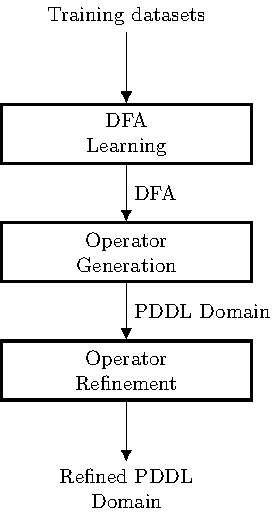
\includegraphics[width=.9\linewidth]{pics/out/amlsi_steps.pdf}
        \caption{AMLSI: {\sf PDDL} domain learning overview}
        \label{fig:contributions:pddl}
    \end{subfigure}
    \begin{subfigure}[b]{.4\linewidth}
        \centering
        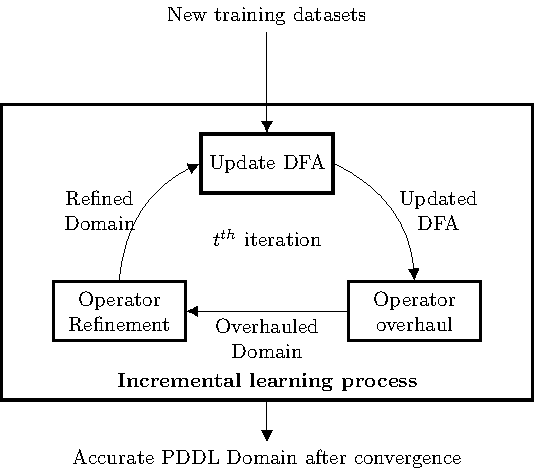
\includegraphics[width=.9\linewidth]{pics/out/incremental_amlsi.pdf}
        \caption{IncrAMLSI: Incremental {\sf PDDL} domain learning overview}
        \label{fig:contributions:incremental}
    \end{subfigure}
    \begin{subfigure}[b]{0.2\linewidth}
        \centering
        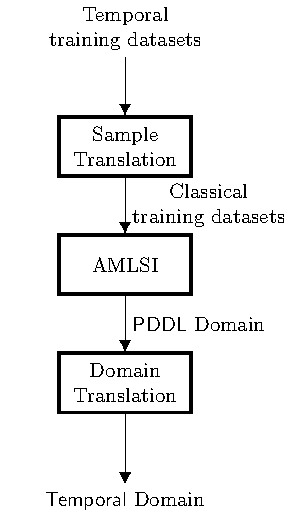
\includegraphics[width=.9\linewidth]{pics/out/temporal_amlsi.pdf}
        \caption{TempAMLSI: {\sf Temporal} domain learning overview}
        \label{fig:contributions:temporal}
    \end{subfigure}
    \caption{Contributions overview}
    \label{fig:contributions}
\end{figure*}

\subsection{Observation Generation}

AMLSI produces a set of observations by using a random walk. AMLSI is able to efficiently exploit these observations by taking into account not only the fact that some actions are applicable in certain states but also that others are not. More precisely, to generate the observations, AMLSI uses random walks by applying a randomly selected action to the initial state of the problem. If this action is feasible, it is appended to the current action sequence. This procedure is repeated until the selected action is not feasible in the current state. The feasible prefix of the action sequence is then added to the set of positive samples, and the complete sequence, whose last action is not feasible, is added to the set of negative samples. This generation method allow to maximize data usability in situations where obtaining training datasets is costly and/time-consuming.

\subsection{Domain Learning}

\paragraph{PDDL Learning}
An overview of the AMLSI \cite{amlsi_ictai, amlsi_keps} algorithm is shown in Figure~\ref{fig:contributions:pddl}. AMLSI is composed of three steps:
\begin{enumerate}
    \item {\em DFA Learning:} AMLSI uses an alternative version of the AMLSI algorithm with the DFA learning algorithm proposed by \cite{amlsi_ictai}.
    \item {\em Operator Generation:} AMLSI generates the set of PDDL operators from the learned grammar DFA with the observed states.
    \item {\em Operator Refinement:} AMLSI refines the operator preconditions and effects. This refinement steps is necessary to address partial and noisy observations.
\end{enumerate}

\paragraph{Incremental Learning}
An overview of the IncrAMLSI algorithm \cite{incr} is shown in Figure~\ref{fig:contributions:incremental}. IncrAMLSI learns incrementally the PDDL domain from incoming data and does not restart from scratch when new data become available at each iteration $t$. More precisely, IncrAMLSI consists in incrementally updating the PDDL domain with the new incoming training datasets available at iteration $t$ to produce the new domain. This algorithm is made up of three steps:
    \begin{enumerate}
        \item {\em Update of the DFA (regular grammar)} with the DFA learning algorithm proposed by \cite{amlsi_ictai}.
        \item {\em Overhaul of the PDDL operators} in order to add new operators and remove preconditions and effects that are no longer compatible with positive and negative samples, and the updated DFA at iteration $t$.
        \item {\em Refinement of the PDDL operators} as in AMLSI algorithm to deal with noisy and partial states in observations.
    \end{enumerate}
The incremental process is operated each time new training datasets are input and until convergence of the PDDL domain.

\paragraph{Temporal Learning}
Some planners, such as Crikey \cite{crikey}, solve {\sf Temporal }Problems by using non-temporal planners. To that end, they convert {\sf Temporal }Problems into {\sf PDDL} planning problems, solve them with a non-temporal planner. Then they convert the classical plan into a temporal plan with rescheduling techniques. TempAMLSI \cite{temp} reuse this idea in order to learn {\sf Temporal} domains: TempAMLSI learns a {\sf PDDL} domain and then infer a {\sf Temporal } domain. TempAMLSI (summarized in Figure \-- \ref{fig:contributions:temporal}) has three steps.
\begin{enumerate}
    \item {\em Sample Translation:} After having generated the samples of {\it temporal} sequences (including both feasible and infeasible sequences), TempAMLSI translates them into non-temporal sequences.
    \item {\em PDDL Domain Learning:} TempAMLSI uses AMLSI to learn an intermediate and classical {\sf PDDL} domain.
    \item {\em Domain Translation:} TempAMLSI translates the PDDL domain into a {\sf Temporal} domain.
\end{enumerate}
This algorithm is able to learn both Sequential and SHE accurate {\sf Temporal} domains.


\section{Document Organization}


\part{Literature Review}
\chapter{Automated Planning}
\minitoc

\chapter{Regular Grammar Induction}
\minitoc

\chapter{Action Model Acquisition}
\minitoc


\part{Contributions}
\chapter{AMLSI \-- STRIPS Domain Learning}
\minitoc

\chapter{Incremental Learning}
\minitoc

\chapter{ADL Domain Learning}
\minitoc

\chapter{Temporal Domain Learning}
\minitoc

\chapter{HTN Domain Learning}
\minitoc


\chapter{Conclusion \& Futur Work}


\part*{Annexes}

\nocite{*}
\bibliographystyle{ieeetr}
\bibliography{biblio,grammar,ml_techniques,soa}
% \nocite{*}
%\printnomenclature
% \listoffigures
% \listoftables
%\nomenclature{$\Sigma$}{Un alphabet}
\nomenclature{$Q$}{Un ensemble d'états}
\nomenclature{$F$}{Un ensemble d'état finaux}
\nomenclature{$\delta$}{Une fonction de transition}
\nomenclature{$q_0$}{Un état initial}
\nomenclature{$q$}{Un état}
\nomenclature{$A$}{Un automate}
\nomenclature{$L$}{Un langage}
\nomenclature{$L(A)$}{Le langage accepté par $A$}
\nomenclature{$\pi$}{Une partition}
\nomenclature{$\lambda$}{Une séquence vide}
\nomenclature{$S_P(L)$}{L'ensemble des préfixes courts}
\nomenclature{$N(L)$}{le noyau d'un langage}
\nomenclature{$I^{+}$}{Un échantillon positif}
\nomenclature{$I^{-}$}{Un échantillon négatif}
\nomenclature{$A(L)$}{L'automate canonique du langage $L$}
\nomenclature{$PTA(I_+)$}{L'arbre accepteur des préfixes}
\nomenclature{$MCA(I_+)$}{L'automate canonique maximal}
\nomenclature{$UA$}{L'automate universel}
\nomenclature{$IS$}{L'état initial d'un problème de planification}
\nomenclature{$G$}{Le but d'un problème de planification}
\nomenclature{$\rho_o$}{La pré-condition d'un opérateur $o$}
\nomenclature{$\epsilon_o$}{Les effets d'un opérateur $o$}
\nomenclature{$\epsilon_o^{+}$}{Les effets positifs d'un opérateur $o$}
\nomenclature{$\epsilon_o^{-}$}{Les effets négatifs d'un opérateur $o$}
\nomenclature{$\Phi_o$}{Les paramètres d'un opérateur $o$}
\nomenclature{$P$}{Un ensemble de prédicats}
\nomenclature{$A^{*}$}{L'automate à apprendre}
\nomenclature{$D$}{Un domaine de planification}
\nomenclature{$D^{*}$}{Le domaine de planification à apprendre}
\nomenclature{$S$}{Une séquence d'actions}
\nomenclature{$B$}{La blackbox}
\nomenclature{$R$}{Un ensemble de contraintes par paires}
\nomenclature{$\mu$}{Un fonction de mapping}
\end{document}
% end of file template.tex
